\documentclass[a4paper,12pt]{article}
\usepackage{pdfpages,cite,hyperref}
\usepackage{natbib}
\usepackage[top=1in, bottom=1.5in,left=1in, right=1in]{geometry}
\setcounter{tocdepth}{2}
\usepackage[utf8]{inputenc}
\usepackage[T1]{fontenc}
\usepackage{lmodern}
\usepackage{caption}
\usepackage{fancyhdr}
\usepackage{array}
\usepackage{subcaption}
\usepackage{enumitem}
\usepackage{tocloft}
\usepackage{setspace}
\linespread{1}
\setlist{nolistsep}
\setlength\cftparskip{8pt}
\setlength\cftbeforesecskip{1pt}
\setlength\cftaftertoctitleskip{2pt}
\bibliographystyle{agsm}
\hypersetup{colorlinks=true,citecolor=blue,linkcolor=blue,filecolor=blue,urlcolor=blue}
\newcolumntype{L}[1]{>{\raggedright\let\newline\\\arraybackslash\hspace{0pt}}m{#1}}
\newcolumntype{C}[1]{>{\centering\let\newline\\\arraybackslash\hspace{0pt}}m{#1}}
\newcolumntype{R}[1]{>{\raggedleft\let\newline\\\arraybackslash\hspace{0pt}}m{#1}}
\pagestyle{fancy}
\fancyhead{}
\fancyfoot{}
\lhead{}
\fancyfoot[LE,RO]{\slshape \rightmark}
\fancyfoot[LO,RE]{\slshape \leftmark}
\lfoot{}
\rfoot{\thepage}
\renewcommand{\footrulewidth}{0.4pt}
\renewcommand{\refname}{Reference List}
\begin{document}
\renewcommand{\headheight}{15pt}
\setlength{\parskip}{\baselineskip}%
\setlength{\parindent}{0pt}%
\pagenumbering{arabic}
\begin{center}
  \vspace*{60mm}
  {\Large \bfseries{AOS Group 3 - SOS Design Documentation}}\\[8mm]
  19$^{th}$ October, 2015\\[20mm]
\end{center}
\newpage
\tableofcontents
\newpage
\section{Overview}
The Simple Operating System, or SOS, performs resource management for
applications running on top of the seL4 Microkernel on ARMv7, specifically the
SABRE Lite i.MX6.  This document describes the design of SOS as implemented by
AOS Group 3.  For each key design choice in the project, it also discusses
benefits and trade-offs of the decision, and possible alternative approaches.
Refer to Doxygen documentation for implementation-specific details and
conventions.

There are 4 distinct problem-areas that have been explored in SOS: the
architecture and execution model, system memory and swapping, processes and
virtual addresses and I/O and drivers.  Understanding the architecture of SOS,
the event loop and syscall dispatch are essential for understanding subsequent
discussions, and thus offers a solid starting point for introducing SOS.

\section{Architecture}
\subsection{Execution Model}
\subsubsection{Design}
Implemented in: \texttt{/apps/sos/src/main.c}

At its core, SOS uses an event-based model implemented using
\emph{continuations}.  A continuation allows for non-blocking behaviour during
otherwise by blocking in a single-threaded implementation (for example I/O) by
providing a way to preserve execution state, thereby maximising the time where
SOS is able to accept new client requests.  This allows for a single-threaded
implementation, while preserving many of the performance characteristics of a
multi-threaded implementation.

A continuation is used to track the current state of execution, including for
example, the original syscall number or fault address and the number of bytes
read or written during the current entry to the kernel.  A continuation is
unique to each \emph{process}.  This model allows execution to resume once an
interrupt occurs, and thus permits SOS non-blocking I/O.

\subsubsection{Discussion}
While a multi-threaded kernel does offer performance advantages on SMP-capable
hardware through the virtue of being able to serve multiple processes
simultaneously, the benefits of multi-threading in a kernel are somewhat
diminished.  There are two reasons for this: the first of which is locks,
which limit scalability, the second of which is that time spent in the kernel
should be designed such that it is minimised.  Thus this is primarily a
concern for high performance applications.  SOS, while designed for
efficiency, is not intended for high performance applications.  On ARM, seL4
is uniprocessor-only and thus a single-threaded implementation may offer
improved performance over a threaded implementation due to the costs imposed
by locking.

The implementation of continuations in SOS is conceptually simple, and allows
for type-checking at compile-time, which affords some correctness guarantees.
However, this struct becomes exceedingly large as more behaviours are added to
SOS, each of which may depend on and need to extend upon the state already
stored in the continuation.

Yet more sophisticated data structures could also be used, which are amenable
to both static analysis or better scalability, such as a hash-table, though to
achieve both static analysis and scalability requires a yet more sophisticated
data structure which imposes added complexities outweighing the benefits
offered to the current incarnation of SOS.

\subsection{Events}
Implemented in: \texttt{/libs/libclock/src/main.c}

\subsubsection{Design}
The \texttt{event\_loop()} serves as the central point of dispatch within SOS, and
services three different forms of events:

\begin{enumerate}
\item Ready Processes
\item Interrupts
\item System Calls
\end{enumerate}

Network and Timer interrupts may come over Asynchronous IPC.  The behaviour
for these will be described in their respective sections later in the
document.  System Calls are received from processes, and will be discussed in
depth in the following section.

Ready processes are serviced before either Interrupts or System Calls.
Processes are enqueued by interrupt handlers: once an interrupt request on
behalf of the process is complete, that process is queued for selection in the
event loop.  Conversely, it can be indicated that a continuation is waiting on
an interrupt through the use of \texttt{longjmp} to \texttt{ipc\_event\_buf},
re-entering the event loop.

At the completion of a client request, the function
\texttt{syscall\_end\_continuation()} is used to reply to the client in a
consistent manner, ensuring that all execution state is released and reset
appropriately.  The caller to \texttt{syscall\_end\_continuation} indicates
the process to reply to, the return code, and whether or not the request was
successful.  At the completion of a request, the state of the process'
continuation is reset.

\subsubsection{Discussion}
The choice of servicing `ready' processes prior to Sync or Async IPC allows
SOS to maximise the number of concurrent I/O operations `in flight': instead
of potentially serving I/O interrupts, we potentially spawn new I/O
interrupts.  Scheduling such that I/O operations are prioritised is known to
allow for higher performance.

\subsection{System Calls}
Implemented in: \texttt{/apps/sos/src/handler.c}, \texttt{/apps/sos/src/syscall.c}

\subsubsection{Design}
As this is a continuation-based model, each syscall is implemented in two
parts: a setup handler, and an execution handler.  The setup handler is called
once, at the beginning of a syscall and before the execution handler is
invoked.  This allows a single, consistent means of storing any arguments
provided via IPC within the continuation, so that they may be available to the
execution handler.

The syscall dispatch is represented as a table which is indexed by the system
call number and the handler type, giving simple and constant-time access to
the syscalls implemented within SOS.

During the execution of a system call, two concepts are used to access the
current current state:
\begin{description}
\item[current\_process] The process which invoked the current system call.
\item[effective\_process] The process which SOS is acting on behalf of.  This
  is usually identical to current\_process, with the exception being spawning
  a child process.  It is defined in terms of the current process.
\end{description}

\subsubsection{Discussion}
The approach to splitting the setup and execution handler for the syscalls
proved largely successful and simplified the implementation substantially.  However,
within the execution handler, the approach to continuations whereby numerous
restartable code-blocks may be contained in a single function, could prove
challenging to debug.

Extending this concept across the entirety of the continuation, whereby a
continuation would contain a list of outstanding execution events which may
(or may not) be required to satisfy each syscall could be a viable approach
and simplify both the syscall implementation, and the continuation structure.
Currently many fields in the continuation denote execution state, and this
approach would allow that state of execution to be separated from other state
and represented consistently.

The downside of this approach would be that the linked list largely becomes a
complex representation of a function call.

\section{System Memory}
\subsection{Frame Table}
Implemented in: \texttt{/apps/sos/src/frametable.c}
\subsubsection{Design}
The frame table is the representation of physical memory. This memory is
mapped by applications and also used by SOS.  Only frames are represented by
the frametable, with other datatypes residing elsewhere in the system.

The frame table is an array of structs, where each struct contains the details
specific to the frame (namely, its address and CPtr), as well as a pointer to
the next element.  When SOS bootstraps, all elements of the array are
allocated, and the free pointer chains each node to its successor.

This structure contains as a list of free frames: as frames are allocated,
they are taken from the head of the list, and as they are freed, they are
returned to the head of the list.  Thus giving a O(1) performance for
allocation and de-allocation of frames.  Similarly, as the structure is an
array, it also offers O(1) lookup as the address can be transformed in to an
index into the array trivially.

\subsubsection{Discussion}
During booting, the frame table is allocated in full, with typed frames for
the frame table being allocated `within' the frame table during allocation.
As the data-structure is 12 bytes in size under the target architecture, this
results in approximately 768 frames of memory being consumed per GiB of
physical memory, delaying boot time.

Furthermore, as the data-structure for a frame doubles to provide pointers to
the next free element, under high memory contention situations approximately
1/3 of the frame table size will be used to store NULL pointers.  Improving
the representation of the frame table would allow for another 256 frames to be
made available for use per GiB of memory.  However, equates to 1MiB of memory
per GiB, which is not significant for most applications.

\subsection{Swap File}
Implemented in: \texttt{/apps/sos/src/frametable.c}

\subsubsection{Design}
When the system encounters contention for the available physical memory
resources, some memory may be swapped to disk.  The data structure which
underpins the swap file is similar to that which underpins the frame table: an
array whose free nodes form a linked list, and as such also offers constant
time lookup, allocation and deallocation.

When reading data from the swap file, or otherwise freeing it, the swap file
is not altered.

The swap structure also features a check-sum field to protect against altered
or corrupted data from being read-in from disk.

\subsubsection{Discussion}
As the swap file is very similar in design to the frame table, it has many of
the same drawbacks.  The structure representing a swap file uses 8 byte nodes,
yielding 512 frames consumed per GB of swap.

While pre-allocing the frame table could be argued for: the memory it consumes
would be consumed anyway, and it trades off boot time performance for run-time
performance, this argument cannot be made with the swap file.  Indeed, the
system may be forced to perform swapping due to the frames occupied by the
data-structure representing the swap file.

A preferable solution would be the use of a data structure which allocated
memory in frames on demand, which could be represented as a two-level `page
table'.  However, such an approach would fix the size of the swap file which
may be a yet more significant issue on systems with restricted disk space or
where the size of the swap file should otherwise be restricted.

\section{Processes and Virtual Memory}
\subsection{Process Management}
Implemented in: \texttt{/apps/sos/src/process.c}, \texttt{/apps/sos/src/elf.c}

\subsubsection{Design}
The design for Process IDs allows for constant-time creation, lookup and
removal, and will reuse process IDs minimally.  This is achieved via an array
of `PID entries', where a PID entry is a double-linked node containing a
process ID and a flag to indicate whether it corresponds to a running process.

Closely related to the use of process IDs is the means by which a process is
identified during a callback.  SOS accounts for potential race conditions by
using a reference to a `callback' structure, which contains the creation time
of the callback, and the PID corresponding to the process which the callback
was created on behalf of.  Given that the creation time of the process is
known, it can be determined whether the process now owning the PID for the
callback is the currently running process; a process starting after the
creation time of the callback cannot own the callback, and thus the callback
is discarded.

\subsubsection{Discussion}
Neither the PID nor the running flag are strictly required.  A PID could
equally have been derived via pointer arithmetic between the beginning of,
and the current index of the table.  Similarly the running flag could be
derived via a lookup into the process table.  However this does afford the
opportunity to verify the correctness of data structure manipulation, and
clarifies the implementation.

\subsection{Page Table}
Implemented in: \texttt{/apps/sos/src/addrspace.c}

\subsubsection{Design}
SOS implements a two-level page table within a process' address space.  The
page table divides the virtual address as follows:

\begin{figure}[h!]
  \centering
  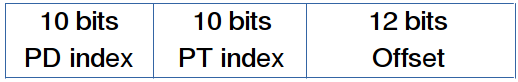
\includegraphics[width=80mm]{add-format.png}
  \caption{Address Format for Page Table lookup}
\end{figure}

This scheme allows each the Page Directory and the second level of the Page
Table to address 1024 4-byte entries within one 4096-byte frame: each 4-byte
entry is a pointer to a Page Table Entry.

A Page Table Entry (PTE) stores the frame address and page cap corresponding
to the virtual address.  As only 20 bits of the frame address are actually
used, the lower 12 bits in the PTE are available for other purposes.
Currently, 3 of these lower-most bits are used to provide flags indicating:
whether the page data is stored on-disk, whether the page is pinned, and
whether it has been referenced.  (See `Page Replacement' for details.)

\begin{figure}[h!]
  \centering
  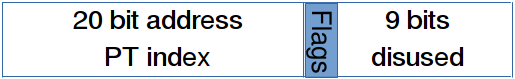
\includegraphics[width=80mm]{pte-addr-format.png}
  \caption{Address Format as stored in the Page Table Entry}
\end{figure}

This structure allows for efficient lookup: the upper 10 most bits index into
the Page Directory, the next upper 10-most bits index in to the second level
of the Page Table.

A linked list is used as the size of a seL4 Page Directory and seL4 Page Table
are 12 and 8 bits respectively, and thus do not map cleanly in to the SOS Page
Table design.  However the data stored in the linked list never need be
accessed explicitly, and exists only for the purpose of releasing the
resource.  A linked list provides constant-time insertion while providing a
simple design at the time of releasing the resources.

\subsection{Page Replacement}
\subsubsection{Design}
SOS implements a second-chance local page replacement algorithm, which takes
place over a number of steps, and occurs in the event that there are isn't any
frames available in the frame table to allocate to a process.

\begin{enumerate}
\item Select the process from which to evict a page.
\item Select a page from that process using a second chance eviction model.
\item Write the page to the swap file.
\end{enumerate}

Selecting the process to evict from is based on a threshold applied across all
process: whether the process exceeds the average number of `evictable' pages
across all processes.  The first process identified which satisfies this
requirement is selected for eviction, or if there isn't any process satisfying
this requirement, the page is evicted from the process which SOS is acting on
behalf of.

In order to guarantee fairness of the system, the process for which eviction
takes place is tracked, and subsequent selection takes place from the
following process.  Similarly, in order to prevent starvation as a result of
two or more processes competing indefinitely for frames, so that they are able
to make progress while the system is under very high resource constraints, the
algorithm may randomly select the current process for eviction.

The page replacement algorithm uses a circular linked list of pages.  For each
page, if the referenced bit for that page table entry is found to be zero, the
page is selected, otherwise the referenced bit is set to zero and the
algorithm proceeds to the next allocated page.

Pages which are pinned, or already swapped to disk are not considered valid
for selection.  Thus there is the potential that there are no pages in the
process which are valid selection.  In this event, (i.e., the event we iterate
through the list more than twice), the process which SOS is acting on behalf
of is killed in order to relieve the memory contention.

Once a page has been selected, the contents of the frame are written to the
next available location in the swap file.  During the copy, the PTE is marked
as \texttt{pinned}, and so is not valid for subsequent selection.  Finally
once the write is complete the page is marked as \texttt{swapd}, indicating an
address on disk.

\subsubsection{Discussion}
Designing a scheme which maximised the amount of memory available for
eviction, thereby maximising the number of processes available to run on the
system, while preserving fairness received a significant amount of attention.
While evicting from the currently running process, or even its parent, is a
reasonably straight-forward approach neither make effective use of system
resources.  However, if pages were to be evicted from other processes, it must
be done in such a way that two or more processes would not compete for the
same resource indefinitely.

There are three factors to the process selection mechanism which help to
ensure fairness:
\begin{description}
\item[queue-based selection] once a process is assessed for selection, every
  other process on the system will be assessed before assessing that process
  again.
\item[threshold based selection] a process will only be selected should it
  have more than the average number of pages available for eviction
\item[biased towards current\_process] selection is biased towards the current
  process (i.e., the process requesting pages) both by defaulting to this
  process should no other process satisfy the requirements for eviction, and
  by the random chance to select this process, which serves to defeat
  processes endlessly competing for resources
\end{description}

As it is too expensive to consider all pages across all processes for
eviction, it depends upon the correct accounting for the number of pages
available to a process for eviction to calculate the threshold predicate,
exposing the potential for future implementation mistakes.

\subsection{Regions}
Implemented in: \texttt{/apps/sos/src/addrspace.c}, \texttt{/apps/sos/src/handler.c}

\subsubsection{Design}
Regions are implemented as a singly-linked list.  Each region also contains
start, end, rights, and an offset for the starting location of that region in
the elf file.

\subsubsection{Discussion}
There is no optimisation on the lookup cost of a region.  This could be
optimised through the use of a Red-Black tree or similar data structure,
though is unnecessarily complex more most applications.

\subsection{Page Faults}
Implemented in: \texttt{/apps/sos/src/handler.c}

\subsubsection{Design}
Page faults within SOS occur in a number of circumstances:

\begin{itemize}
\item for lazy-loading data in from an ELF binary;
\item faulting-in new pages within the heap or stack, and
\item when the process attempts to read data, which has been paged to disk, back into memory;
\item as a means of setting the frame referenced bit for second chance replacement
\end{itemize}

In the event a page corresponding to a virtual address has not been created
within a processes address space when it faults, a new page will be created
dynamically.  When this occurs the corresponding region is used to determine
whether any data should subsequently be loaded in to that page.  This is
indicated by an elf file offset being defined for the corresponding region.
Therefore in this event content for code and data segments will be loaded from
the ELF binary, while zeroed pages will be allocated for the stack and heap as
the process faults within those regions.

Data paged to disk will be indicated by the \texttt{swapd} bit in the corresponding
PTE.  In the event a fault occurs on a page with this bit set, the address
(which corresponds to an offset within the swap file) will be used to read in
the page.  During the read, another page may or may not be evicted depending
on whether physical memory is available to facilitate the replacement.

The final scenario in which page faults will occur is in order to set the
`referenced' bit (\texttt{refd}) of the page to facilitate second-chance page
replacement.  During the replacement algorithm, pages where the referenced bit
is unset will also be unmapped from the process' address space.  Thus when a
fault occurs on a page where the referenced bit is not set, though it is still
in memory, the referenced bit will be set and the page mapped back in to the
process' address space.

\section{I/O and Drivers}
\subsection{IO Vectors}
Implemented in: \texttt{/apps/sos/src/file.c}

\subsubsection{Design}
An IO Vector is a representation of client or SOS-internal pages, allowing
memory to be mapped for I/O on-demand.

An IO Vector provides the following fields:
\begin{description}
\item[vstart] The starting address of the frame or virtual address (conditional)
\item[sz] The length of the operation to occur.  sz will be set such that the
  operation does not exceed the page given the starting address \texttt{vstart}.
\item[next] The following IO Vector node.
\item[sos\_iov\_flag] Flag indicating whether the IO Vector node corresponds to
  a SOS frame, or process virtual address (thereby indicating whether
  address translation is required)
\end{description}

The benefit of the IO Vector is that it allows for otherwise non-contiguous
pages to be treated as though contiguous.  It also provides a means for
representing the progress of an IO operations, where the IO Vector need simply
be updated to reflect the current progress of an operation.  Similarly, we
need only guarantee the page for the current IO Vector is in memory, thus
alleviating the need to read all pages for the current IO operation into
memory.

IO Vectors are used to represent most I/O operations in SOS.

\subsubsection{Discussion}
Currently the usage of the IO Vector means that we may do short IO ops
(e.g. 10 bytes to finish reading a page), even though we could do a large IO
op (4k) and write across IO Vectors simultaneously.  Correcting this would
incur some complexity in the implementation, though also offers the
opportunity for significant performance improvements, in particular when
reading files over NFS.


\subsection{I/O Device Abstraction}
\subsubsection{Design}
The I/O Device is an abstraction over both block and character devices.  In
the case of SOS, this abstracts both Serial and NFS to create a uniform IO
interface through mapping function pointers to their respective
implementations.

Thus an IO Device provides an interface for all available IO operations over
any driver.  Thus it currently exposes:

\begin{itemize}
\item open
\item close
\item read
\item write
\item getdirent
\item stat
\end{itemize}

For both the serial and NFS drivers.  As the serial driver does not support
some of these operations, those operations are undefined (NULL).

\subsubsection{Discussion}
The IO Device is a light-weight mechanism to abstract access to IO-related
drivers.  An alternative to this would be the implementation of a VFS-like
abstraction.  However, given that the goals of the project were to support a
single, flat filesystem, and a serial device, this was deemed an overly
extravagant abstraction.

\subsection{Serial Device}
Implemented in: \texttt{/apps/sos/src/serial.c}

\subsubsection{Design}
The serial device implementation satisfies single-reader / multiple-writer
semantics, where the process is only permitted to read should no other process
have the serial device open for reading.  This uses global state (named
\texttt{reader\_pid}) within the serial driver, which allows the owning process to be
identified in constant time.

Reads in SOS are buffered, though only the most recent line is preserved; any
subsequent line is discarded.  This provides bounds over the size of the
buffer, while allowing non-blocking behaviour should have already been
provided from the user.

When the read() is invoked by the client, the pages corresponding to that read
are pinned, and subsequently unpinned when the read operation returns to the
caller.  As the buffer is at most 1024 bytes, up to two pages can be pinned
because of this.

The serial driver is initialised at boot-time.

\subsection{NFS}
Implemented in: \texttt{/apps/sos/src/sos\_nfs.c}

\subsubsection{Design}
The NFS implementation in SOS relies heavily on callbacks and continuations,
which have been discussed previously.  Prior to spawning a request for which a
subsequent callback is expected, a `callback info' struct will be allocated,
which contains the time the callback was initiated and the process initiating
the callback.  The address of this is used as the token, and uniquely
identifies the context for the callback once the callback is realised.

The PID from the callback is used to set the context for the subsequent
execution, in the same was as the badge for a process' IPC is used to set the
context for a syscall.

Detection of completion of the syscall is handled individually in each
callback.  In the event of error, or completion, the callback is responsible
for triggering an appropriate reply to the client over IPC.

\subsection{Timer Interrupts}
Implemented in: \texttt{/libs/libclock/src/clock.c}

\subsubsection{Design}
The timer interrupt was implemented using the GPT timer on the SABRE.

The GPT timer allows multiple Output Compare Registers to be set
simultaneously, and thus affords the ability to support two different types of
interrupts.

\begin{enumerate}
\item Regular 100ms kernel tick
\item Timed callback events
\end{enumerate}

Both timed callbacks and kernel tick callbacks are exposed via an interface
for registering callback functions when these events occur.

Timed callbacks are called after a timeout expires.  This is implemented by
ensuring that all registrations are ordered at registration-time, and setting
the corresponding Output Compare Register to the next event in the queue.  The
next event in the queue is determined through looking up the next callback in
a array, which is sorted by callback time.  Timer overflow is accounted for by
searching for the event such that the difference between the current time, and
the event time is minimal at the time of registration.

Timed callbacks are removed after being fired and are used to implement the
\texttt{sleep} syscall.  As kernel tick events satisfy different semantics to
timed callback events in the implementation, they are distinguished in the
interface.

\subsubsection{Discussion}
Alternatively the EPIT timer could have been used to implement this
functionality.  Both EPIT and GPT timers on the Sabre have a very similar
interface, and both could equally have been used.  However it was elected that
the GPT is slightly simpler and fulfills all requirements.

The implementation trades-off registration and removal performance for
interrupt performance: registration and removal are both linear time
operations as they ensure the callback timeouts are sorted based on the time
they must trigger.  The interrupt handler offers constant-time performance for
the lookup for the expiring callbacks.

\end{document}
%%% Local Variables:
%%% mode: latex
%%% TeX-master: t
%%% End:
